\chapter {SOFTWARE TESTING}
\section{Introduction}
\subsection{Purpose}
Software testing can be stated as the process of validating and verifying that a computer program/application/product:
\begin{itemize}
\item Meets the requirements that guided its design and development.
\item Works as expected.
\item Can be implemented with the same characteristics.
\item Satisfies the needs of stakeholders.
\end{itemize}

Software testing, depending on the testing method employed, can be implemented at any time in the development process. Traditionally most of the test effort occurs after the requirements have been defined and the coding process has been completed, but in the Agile approaches most of the test effort is on-going. As such, the methodology of the test is governed by the chosen software development methodology.

\subsection{Scope}
The testing of the system was done manually and no testing tools were used. The \emph{test plan} describes the \emph{unit, functional, performance, usability, regression} tests that were performed. Only codes that were pushed as commits were considered as candidates for testing.

\subsection{Intended Audience}
The testing of this system is intended for 3 types of audiences:
\begin{enumerate}
\item \textbf{End Users:} The users who will be using the system will review the testing as a mark of stability and performance of the system.
\item \textbf{Developers:} Will view the testing for knowing existing limitations and bugs.
\item \textbf{Reviewers:} Will use these test results as a metric to evaluate the project.
\end{enumerate}

\section{Test Cases}
\subsection{Introduction}
The purpose of this Test Case document is to specify and communicate the specific
conditions which need to be validated to enable an assessment of the system. Test
Cases are motivated by many things but will usually include a subset of Use Cases,
performance characteristics and the risks the project is concerned with.
A separate test case document is prepared for each testing phase (unit,
integration, integrity, etc.) identified in the test plan. The test cases should be
organised into related groups that are meaningful to the project – i.e. test suites.

\subsection{File System Operations}
Testing the file system for implementations of required operations:
\begin{table}[h]
\begin{tabular}{|p{2cm}|p{2cm}|p{8cm}|}
\hline
\textbf{Operation} & \textbf{Status} & \textbf{Comment} \\ \hline
getattr & YES & checks whether the given path exits \\
readdir	 & YES & lists the contents of the given tag \\
access	& YES & checks for access to specified tag \\
truncate	 & YES & closes file after operation \\
destroy	 & YES & called on file system unmount \\
open		& YES & opens for file for access \\
release	& YES & releases file after access \\
mknod		& YES & creates new file \\
rename		& YES & renames files and folders \\
unlink		& YES & removes file from system \\
read		& YES & reads data from file \\
write		& YES & writes data to file \\
chmod		& YES & changes permissions \\
chown		& YES & changes owner\\
mkdir		& YES & creates new directory \\
rmdir		& YES & removes directory\\

symlink	 & INVALID & not required in KWEST \\ 
readlink & INVALID & not required in KWEST \\
link		& INVALID & not required in KWEST \\
utimens	& NO & not implemented \\
statfs	& NO & not implemented \\
fsync & INVALID & not required in KWEST \\

setxattr	& NO & not implemented \\
getxattr	& NO & not implemented \\
listxattr	& NO & not implemented \\
removexattr	& NO & not implemented \\
\hline
\end{tabular}
\caption{File system operations}
\label{fsop}
\end{table}

\section{Snap shots of the test cases and Test plans}
\section*{Test Plan}
\subsection{Target Items}
The following have been identified as targets for testing:
\begin{enumerate}
\item Code and associated areas
\item File system operations
\item Databases: SQLite3
\item Operating Systems
\end{enumerate}

\subsection{Outline of Tests}
\subsection*{Tests performed}
\begin{enumerate}
\item Performance tests
\item Functional tests
\item Data Integrity tests
\item Regression tests
\item Usability tests
\end{enumerate}

\subsection{Test Approach}
Any bugs found should be reported with related information, which should include
who discovered it, how, a description of the bug, and who fixed it and
when. Also, re-testing of the code done to make sure that defect has been fixed
and there no new bugs produced due to change in code.

\begin{enumerate}
\item \textbf{Performance Testing:} \\
The focus of Performance testing is checking a software program’s
\begin{itemize}
\item \emph{Speed} : Determines whether the system responds quickly.
\item \emph{Scalability} : Determines maximum user load the software application can handle.
\item \emph{Stability} : Determines if the application is stable under varying loads.
\end{itemize}
\textbf{Tools required:} Software timers \\
\textbf{Success criteria:} 
\begin{enumerate}
\item Manual(user) perception does not notice any ``lags''.
\item Time to perform operations is within an acceptable range.
\end{enumerate}


\item \textbf{Functional Testing:} \\
The prime objective of Functional testing is   checking the functionalities of the software system. It mainly concentrates on -
\begin{itemize}
\item \emph{Mainline functions} :  Testing the main functions of an application.
\item \emph{Basic Usability} : It involves basic usability testing of the system. It checks whether an user can freely navigate through the screens without any difficulties.
\item \emph{Accessibility} :  Checks the accessibility of the system for the user.
\item \emph{Error Conditions} : Usage of testing techniques to check for error conditions.  It checks whether suitable error messages are displayed.
\end{itemize}
\textbf{Tools required:} None(manual testing) \\
\textbf{Success criteria:} All of the following are successfully tested:
\begin{enumerate}
\item all key use-case scenarios.
\item all key features.
\end{enumerate}

\item \textbf{Data Integrity Testing:} \\
Data integrity refers to the quality of the data in databases and is the measurement by which users examine data quality, reliability and usefulness. Data integrity testing verifies that converted data is accurate and functions correctly within a given application. Testing data integrity involves:
\begin{itemize}
\item \textbf{Database} : Verifying that correct values are saved in databases.
\item \textbf{Write-back} : Correct data is written to disk.
\item \textbf{Read} : Correct data is read from disk.
\item \textbf{File Integrity} : Operations do not break existing files.
\end{itemize}
\textbf{Tools required:} File compare tools (manual testing) \\
\textbf{Success criteria:} All of the following are successfully tested:
\begin{enumerate}
\item files are same in size, byte-blocks, permissions and parameters.
\item data is not changed, modified or removed unless intended.
\end{enumerate}

\item \textbf{Regression Testing:} \\
Regression Testing is required when there is a :
\begin{itemize}
\item Change in requirements and code is modified according to the requirement
\item New feature is added to the software
\item Defect fixing
\item Performance issue fix 
\end{itemize}
\textbf{Tools required:} None(manual testing) \\
\textbf{Success criteria:} All of the following are successfully tested:
\begin{enumerate}
\item all previous operations are successfully executed.
\item previously solved bugs are not re-introduced.
\item operations do not suffer from unwanted performance hits.
\end{enumerate}

\item \textbf{Usability Testing:} \\
Goal of this testing is to satisfy users and it mainly concentrates on the following parameters of a system: \\
\textbf{Effectiveness of the system}
\begin{itemize}
\item Is the system is easy to learn?
\item Is the system useful and adds value to the target audience?
\item Is Content, Colour, Icons, Images used are aesthetically pleasing ?
\end{itemize}
\textbf{Efficiency}
\begin{itemize}
\item Navigation required to reach desired screen/web page should be very less. Scroll bars shouldn’t be used frequently.
\item Uniformity in the format of screen/pages in your application/website.
\item Provision to search within your software application or website
\end{itemize}
\textbf{Accuracy}
\begin{itemize}
\item No outdated or incorrect data like contact information/address should be present.
\item No broken links should be present.
\item User Friendliness
\item Controls used should be self-explanatory and must not require training to operate
\item Help should be provided for the users to understand the application / website
\item Alignment with above goals helps in effective usability testing
\end{itemize}
\textbf{Tools required:} None(manual testing) \\
\textbf{Success criteria:} All of the following are successfully tested:
\begin{enumerate}
\item operations are not changed drastically from a traditional file system.
\item user can use the file system without any special tools.
\end{enumerate}
\end{enumerate}

\subsection{Entry and Exit Criteria:}

\begin{enumerate}
\item Test Plan
\begin{enumerate}[label=\Alph*]
\item \textbf{Test Plan Entry Criteria:} Code is complete and has been pushed to the Git repository.
\item \textbf{Test Plan Exit Criteria:} All functional requirements have been verified.
\item \textbf{Suspension and Resumption Criteria:} Testing will be suspended on critical
design flaws that will changes in redesign of critical components. Testing will resume when the coding is complete and code is reviewed successfully.
\end{enumerate}

\item Test Cycle
\begin{enumerate}[label=\Alph*]
\item \textbf{Test Cycle Entry Criteria:} When a module has been completed.
\item\textbf{ Test Cycle Exit Criteria:} All tests specified at the start of the testing have
completed successfully.
\end{enumerate}
\end{enumerate}

\subsection{Risks, Dependencies, Assumptions, Constraints}
\begin{table}[h]
\begin{tabular}{|p{2cm}|p{8cm}|p{4cm}|}
\hline
\textbf{Risk} & \textbf{Mitigation Strategy} & \textbf{Contingency} \\ \hline
FUSE API changes & Use FUSE version numbers to run a static check while compiling for required version of FUSE. & Change operation code to new version. \\ \hline
External Library is no longer maintained & Try to use the latest version number of library available and keep a source ready for distribution. & Change to alternate library. \\ \hline
Performance has degraded & Code with performance in mind, using fast algorithms and approaches. & Use profiling tools to detect memory issues and static code analysers for code checking. \\
\hline
\end{tabular}
\caption{Risk Management}
\label{tab: risk}
\end{table}

\subsection{Problem Reporting, Escalation, and Issue Resolution}
Each bug will be given a priority, which will determine when it is addressed in the current iteration. The bug priority may change due to other bugs, issues or re-evaluation of the bug by a peer review.

\section*{SNAP SHOTS OF TEST CASES}
%insert screenshots here
\subsection{File system operation testing}
There are no good tools for exhaustively testing file system operations for reliability, freedom from bugs, scalability, etc. Often file system developers will use some scripts to run various operations such as creating and deleting files. The best known tool for testing file systems is called SPEW, which will thoroughly test a small subset of file system operations concerning the mix of read/write operations, memory-mapped operations, and file truncation operations, all inside a single file. None of the existing solutions covers all file system operations.

\newpage
\subsubsection{Testing file system for ghost accesses}
\begin{figure}[htb]
\centering
\setlength\fboxsep{0pt}
\setlength\fboxrule{0.5pt}
\fbox{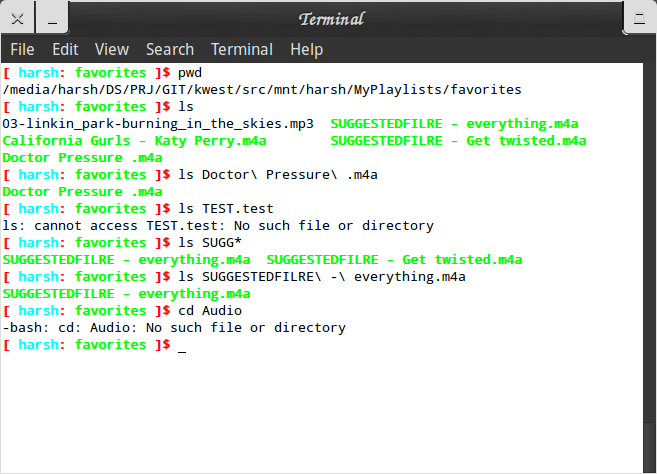
\includegraphics[width=0.8\linewidth]{./testcases/tc01.png}}
%\includegraphics[width=0.8\textwidth]{image.png}
\caption{Accessing non-existant entries on file system}
\label{fig:dfd0}
\end{figure}
The above screenshot depicts access to a non-existant file \emph{TEST.txt} and directory \emph{Audio}. Both are not present in the current folder. The bash terminal error displayed is \emph{No such file or directory}.

\subsubsection{Copying suggestions}
\begin{figure}[htb]
\centering
\setlength\fboxsep{0pt}
\setlength\fboxrule{0.5pt}
\fbox{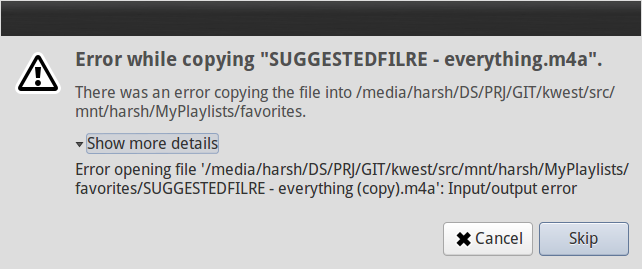
\includegraphics[width=0.8\linewidth]{./testcases/tc02.png}}
%\includegraphics[width=0.8\textwidth]{image.png}
\caption{Error shown while copying suggestions}
\label{fig:dfd0}
\end{figure}
Suggestions are virtual entities which cannot be copied to another folder. However, the file represented by it can be opened and used as any normal file. The error shown was displayed in the \emph{Nemo} file manager.

\subsubsection{Copying files within different mime types}
\begin{figure}[htb]
\centering
\setlength\fboxsep{0pt}
\setlength\fboxrule{0.5pt}
\fbox{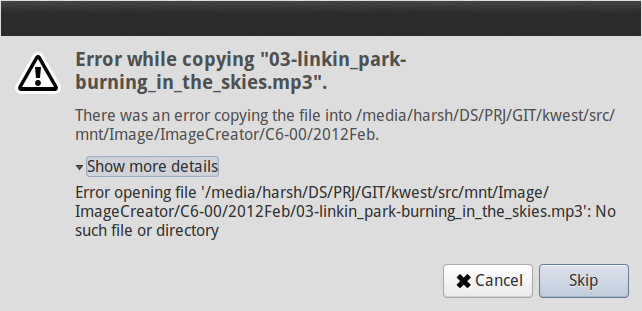
\includegraphics[width=0.8\linewidth]{./testcases/tc03.png}}
%\includegraphics[width=0.8\textwidth]{image.png}
\caption{Error shown while copying an Audio file to Images}
\label{fig:dfd0}
\end{figure}
Files can only be moved within their own mime types and within user tags. Putting an audio file in an image folder is not allowed. The error shown above was displayed in the \emph{Nemo} file manager.

\subsubsection{Copying system generated folders}
\begin{figure}[htb]
\centering
\setlength\fboxsep{0pt}
\setlength\fboxrule{0.5pt}
\fbox{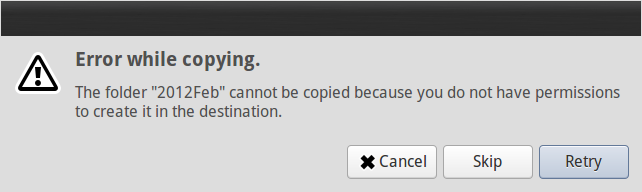
\includegraphics[width=0.8\linewidth]{./testcases/tc04.png}}
%\includegraphics[width=0.8\textwidth]{image.png}
\caption{Copying an image folder representing `date'}
\label{fig:dfd0}
\end{figure}
The folders are generated by the system depending on the meta-data of the files displayed under them. They cannot be moved anywhere other than their correct category. E.g. Audio folders can be moved within artists and albums, but not anywhere else. The error displayed above was taken from the \emph{Nemo} file manager.

\subsubsection{Copying files within KWEST}
\begin{figure}[htb]
\centering
\setlength\fboxsep{0pt}
\setlength\fboxrule{0.5pt}
\fbox{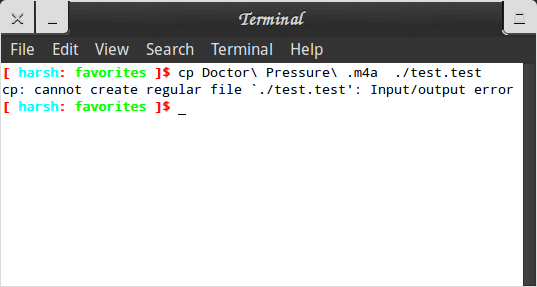
\includegraphics[width=0.8\linewidth]{./testcases/tc05.png}}
%\includegraphics[width=0.8\textwidth]{image.png}
\caption{Creating a copy of the same file in KWEST}
\label{fig:dfd0}
\end{figure}
Copying a file within KWEST is an unsupported operation. This is due to the duplicity of metadata generated by two copies of the same file. In the screenshot, the user tries to create a copy using the \emph{cp} command. KWEST restricts the operation and bash displays the error \emph{Cannot create regular file: input/output error}.

\subsubsection{Renaming files and folders within KWEST}
\begin{figure}[htb]
\centering
\setlength\fboxsep{0pt}
\setlength\fboxrule{0.5pt}
\fbox{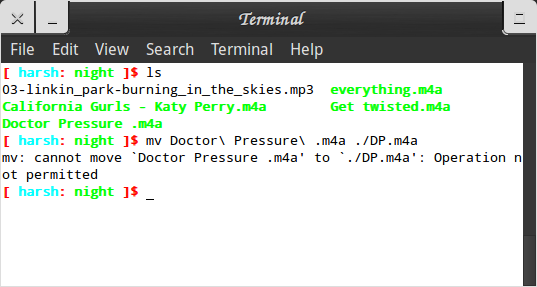
\includegraphics[width=0.8\linewidth]{./testcases/tc06.png}}
%\includegraphics[width=0.8\textwidth]{image.png}
\caption{Renaming an audio file in KWEST}
\label{fig:dfd0}
\end{figure}

\begin{figure}[htb]
\centering
\setlength\fboxsep{0pt}
\setlength\fboxrule{0.5pt}
\fbox{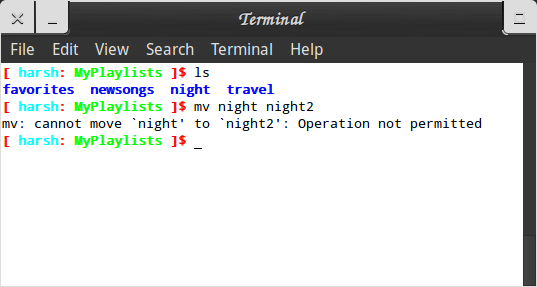
\includegraphics[width=0.8\linewidth]{./testcases/tc07.png}}
%\includegraphics[width=0.8\textwidth]{image.png}
\caption{Renaming a folder in KWEST}
\label{fig:dfd0}
\end{figure}
Files cannot be renamed in KWEST. This is in part due to files being displayed by their metadata contents, and also due to the duplication of metadata in case of renamed files. In the screenshot above a file and a folder are being renamed using the \emph{mv} command. In this case bash returns the error \emph{Operation not allowed} signifying that KWEST does not allow this operation. The \emph{mv} command can still be used for moving files.

\subsubsection{Deleting files in KWEST}
\begin{figure}[htb]
\centering
\setlength\fboxsep{0pt}
\setlength\fboxrule{0.5pt}
\fbox{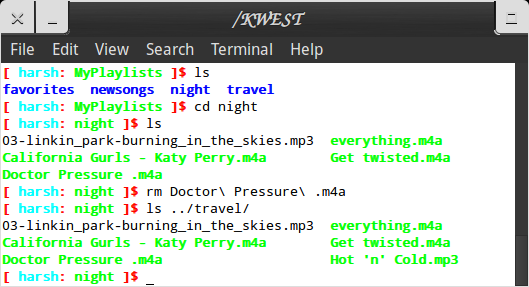
\includegraphics[width=0.8\linewidth]{./testcases/tc12.png}}
%\includegraphics[width=0.8\textwidth]{image.png}
\caption{Removing a file in one tag without affecting other tags}
\label{fig:dfd0}
\end{figure}
A user file can be removed from the current tag without it being deleted from the other tags. The screenshot shows the file \emph{Doctor Pressure.m4a} being removed from the \emph{night} tag while the file is still present in other tags.

\subsubsection{Loops in browsing the file system}
\begin{figure}[htb]
\centering
\setlength\fboxsep{0pt}
\setlength\fboxrule{0.5pt}
\fbox{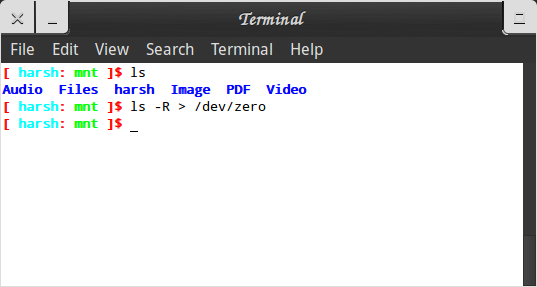
\includegraphics[width=0.8\linewidth]{./testcases/tc08.png}}
%\includegraphics[width=0.8\textwidth]{image.png}
\caption{Listing entries recursively to detect loops}
\label{fig:dfd0}
\end{figure}
A virtual file system having references to multiple parents can have loops where the user can traverse the same set of folders while going \emph{deeper} into the file system heirarchy. The simple terminal test \emph{ls -R} can show whether such loops exist. The end of operation denotes that the terminal was able to traverse all paths and return, signifying that there were no loops in the file system.

\newpage
\subsection{Performance of file system operations}
Comparison of KWEST file system against underlying file system.
\textbf{Test Bench:}
\begin{itemize}
\item Operating System: Linux Mint 14 3.5.0-25-generic
\item Original file system: ext4 500GB disk with partition size 150GB
\item RAM: 4GB
\item swap: 8GB on disk
\item CPU utilisation: average 4%
\end{itemize}
\textbf{Contents of Music folder imported into KWEST:}
\begin{itemize}
\item \textbf{Audio:} 17 files totalling 102.9MB
\item \textbf{Images:} 81 files totalling 196MB
\item \textbf{PDF:} 11 files totalling 17.9MB
\item \textbf{Video:} 4 files totalling 1GB
\item \textbf{Others:} 7 files totalling 7MB
\item \textbf{Total:} 120 files of size 1.3GB
\end{itemize}

\begin{table}[h]
\begin{tabular}{|p{3cm}|p{2cm}|p{7cm}|}
\hline
\textbf{Test} & \textbf{Time taken} & \textbf{Comment} \\ \hline
all files	&	120sec	& total file size imported was 1.3GB \\ \hline
videos	& 40sec	&	extracting metadata from videos is more expensive compared to other file types \\ \hline
images	& 35sec & images having metadata take longer than those without \\ \hline
audio 	& 4sec	& audio files are the fastest to parse and load \\ \hline
PDF		& 2sec	& PDF files are parsed quickly as compared to other document types \\ \hline
forming associations & 2sec	 & time is proportional to number of common files in user tags \\
\hline
\end{tabular}
\caption{Performance tests for mounting KWEST}
\label{performancemount}
\end{table}

\subsubsection{IOZone statistics}
\begin{figure}[htb]
\centering
\setlength\fboxsep{0pt}
\setlength\fboxrule{0.5pt}
\fbox{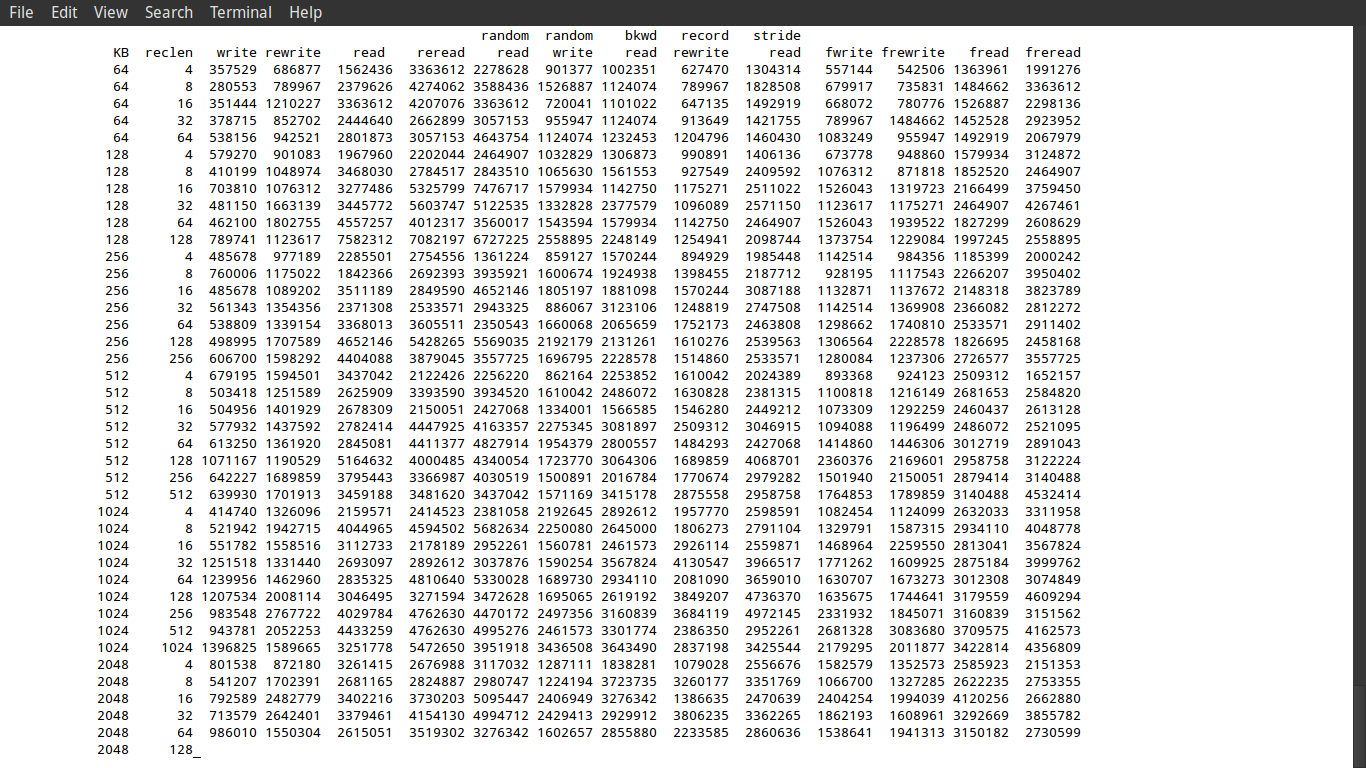
\includegraphics[width=0.8\linewidth]{./testcases/tc09.png}}
%\includegraphics[width=0.8\textwidth]{image.png}
\caption{IOZone statistics for various operations}
\label{fig:dfd0}
\end{figure}
IOzone is a filesystem benchmark tool. The benchmark generates and measures a variety of file operations. Iozone has been ported to many machines and runs under many operating systems.Iozone is useful for performing a broad filesystem analysis of a vendor’s computer platform. The benchmark tests file I/O performance for the following operations: Read, write, re-read, re-write, read backwards, read strided, fread, fwrite, random read/write, pread/pwrite variants. Homepage: \url{http://www.iozone.org/}

\subsubsection{SPEW performance tests on KWEST}
Spew is used to measure I/O performance of character devices, block devices, and regular files. It can also be used to generate high I/O loads to stress systems while verifying data integrity. Spew is easy to use and is flexible. No configuration files or complicated client/server configurations are needed. Spew also generates its own data patterns that are designed to make it easy to find and debug data integrity problems. Homepage: \url{http://spew.berlios.de}.
\begin{figure}[htb]
\centering
\setlength\fboxsep{0pt}
\setlength\fboxrule{0.5pt}
\fbox{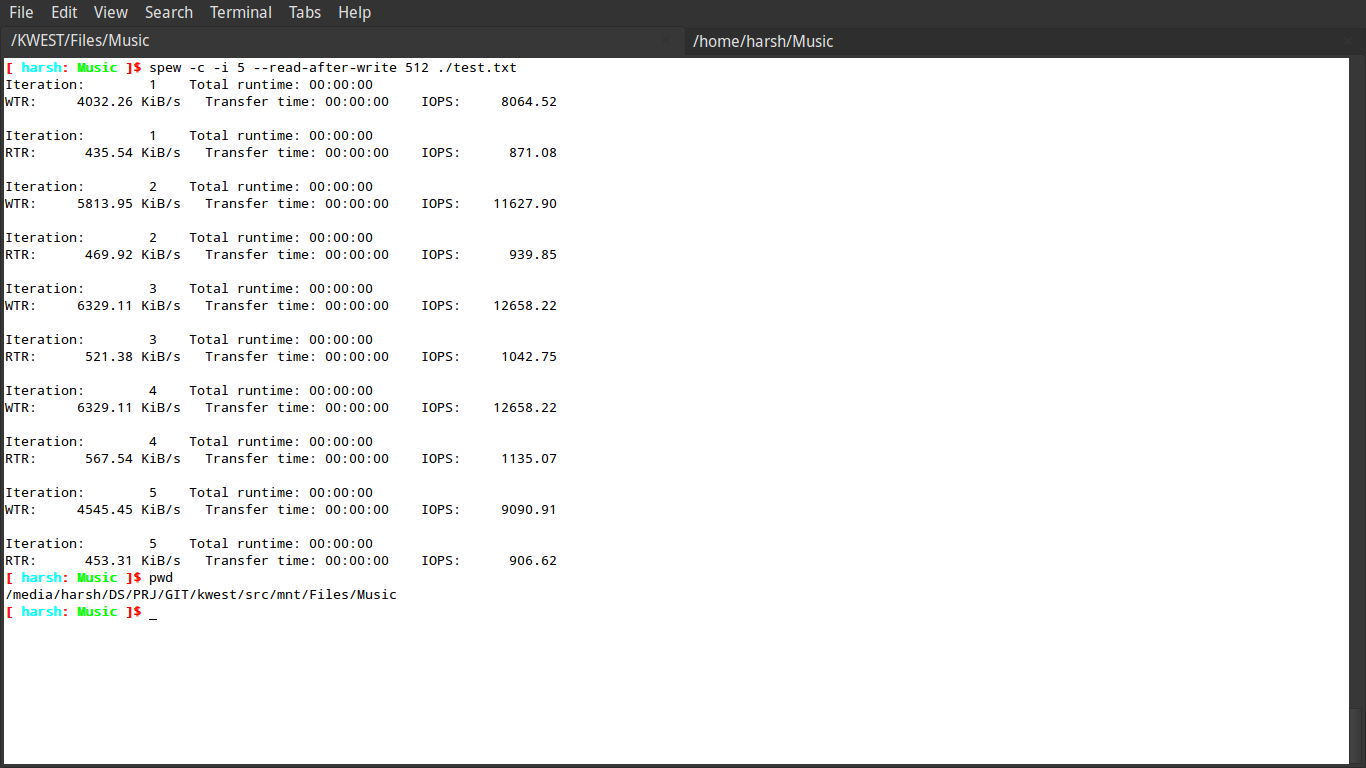
\includegraphics[width=0.8\linewidth]{./testcases/tc10.png}}
%\includegraphics[width=0.8\textwidth]{image.png}
\caption{SPEW performing read-after-write on KWEST}
\label{fig:dfd0}
\end{figure}

\begin{figure}[htb]
\centering
\setlength\fboxsep{0pt}
\setlength\fboxrule{0.5pt}
\fbox{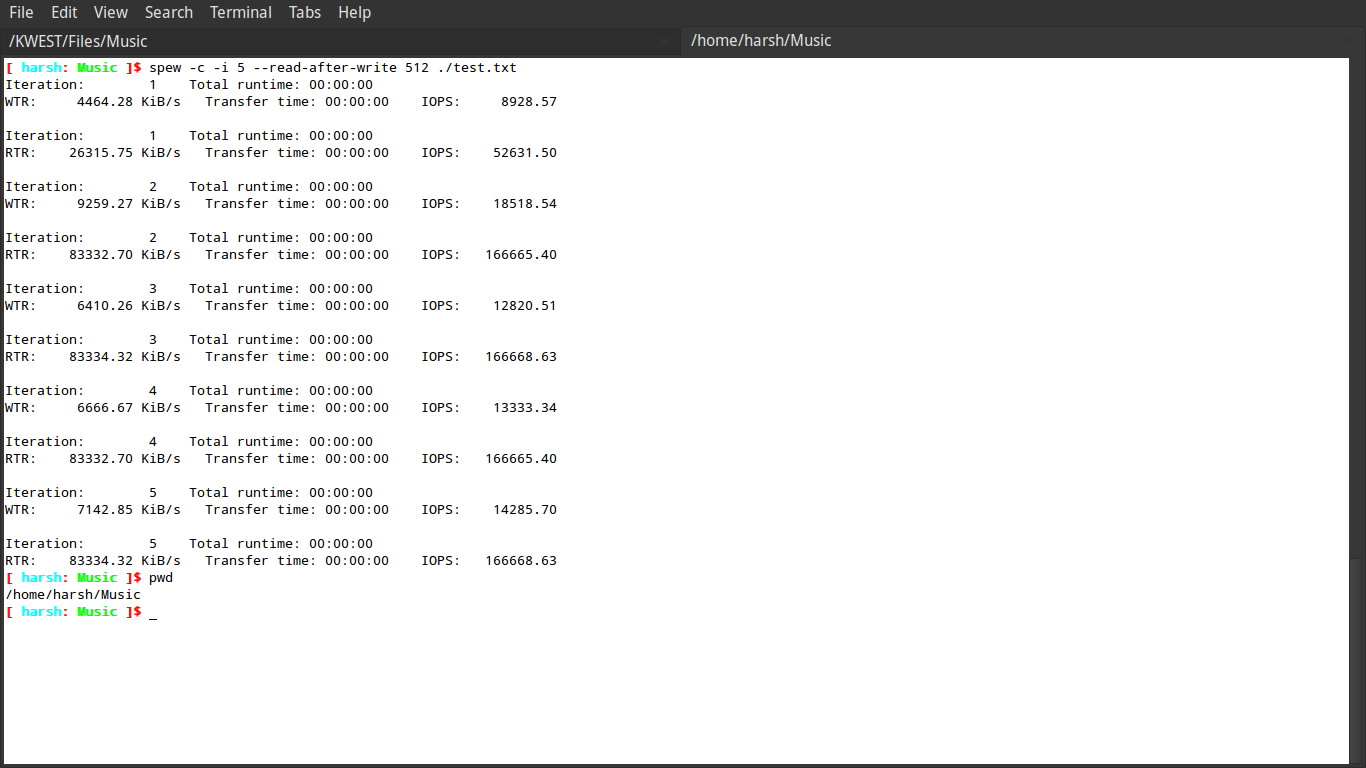
\includegraphics[width=0.8\linewidth]{./testcases/tc11.png}}
%\includegraphics[width=0.8\textwidth]{image.png}
\caption{SPEW performing read-after-write on underlying file system}
\label{fig:dfd0}
\end{figure}
The screenshot depicts the spew read-after-write test which writes random bytes to a file and then performs sequential reads on it. The statistics show that KWEST has a good write data rate which is comparable to regular file systems. However, read rate sees a significant drop. In spite of this, usability tests show that for a regular user, the file system offers satisfactory performance.

\newpage


\subsubsection{Test scripts} 
The following is a simple test script used to evaluate file system operations. The script works by calculating the difference in time before and after the execution of operations.
\begin{lstlisting}[language=bash,frame=single]
#store current time
let DA=(`date +%s `)
#perform file system operation
ls -R kwest/src/mnt
#store new time
let DB=(`date +%s`)
#calculate the difference
let DC=$DB-$DA
#output the time taken
echo $DC
\end{lstlisting}

\begin{table}[h]
\begin{tabular}{|p{2cm}|p{1.5cm}|p{1.5cm}|p{7cm}|}
\hline
\textbf{Operation} & \textbf{ext4} & \textbf{KWEST} & \textbf{Comment} \\ \hline
list directory	&	500ms	&	550ms & there is no noticeable difference \\ \hline
read file	&	700ms & 850ms	& some extra time is taken to read a file depending on the amount of data being read. In general, there is no noticeable difference. \\ \hline
write file	&	1200ms & 2200ms	& (for 5MB text file) writing takes slightly more time, but the difference is within acceptable range. \\ \hline
read and write	&	1010ms & 2400ms & (for 5MB text file) reading and writing simultaneously does not produce any performance degradation. \\
\hline
\end{tabular}
\caption{Performance tests for using KWEST}
\label{performancetests}
\end{table}

\newpage
\subsubsection{READ operation TEST}
Read operation test included reading from a 4.1MB file and outputing the contents on terminal. The file was accessed on the KWEST file system.
\begin{lstlisting}[language=bash,frame=single]
GNU nano 2.2.6              File: ./test.sh                                   
echo "READ test"
echo "cat ./mnt/Files/Music/t2.txt 
let kT=0
for i in 1 2 3 4 5 
do
echo "Run#" $i
#store current time
let kS=(`date +%s`)
#perform file system operation
cat ./mnt/Files/Music/t2.txt > ./mnt/Files/Music/test.txt
#store new time
let kE=(`date +%s`)
#calculate the difference
let kO=$kE-$kS
let kT=kT+kO
#output the time taken
echo "kwest operation time = " $kO "sec"
done
let kT=kT/5
echo "average time taken = " $kT
\end{lstlisting}
\begin{figure}[htb]
\centering
\setlength\fboxsep{0pt}
\setlength\fboxrule{0.5pt}
\fbox{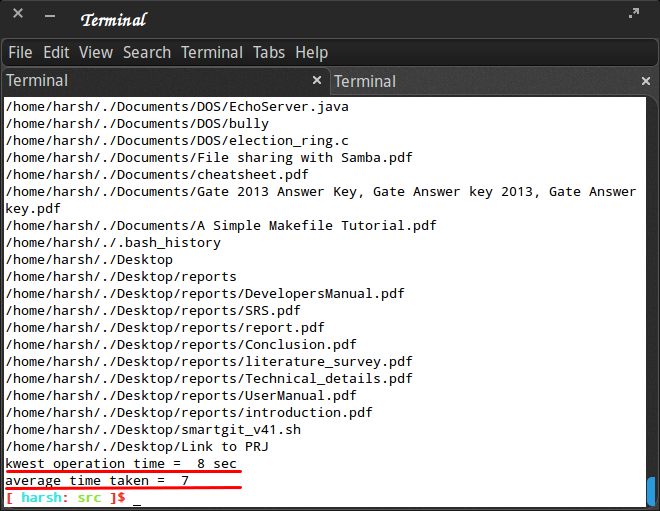
\includegraphics[width=0.8\linewidth]{./opimg/readtest.png}}
%\includegraphics[width=0.8\textwidth]{image.png}
\caption{Read operation average time for 4.1MB text file}
\label{fig:dfd0}
\end{figure}

\subsubsection{WRITE operation test}
Write operation test included reading from a 4.1MB file and writing the contents to another file. Both the files were accessed from the KWEST file system.
\begin{lstlisting}[language=bash,frame=single]
GNU nano 2.2.6              File: ./test.sh        
echo "READ test"
echo "cat ./mnt/Files/Music/t2.txt > ./mnt/Files/Music/test.txt"
let kT=0
for i in 1 2 3 4 5 
do
echo "Run#" $i
#store current time
let kS=(`date +%s`)
#perform file system operation
cat ./mnt/Files/Music/t2.txt > ./mnt/Files/Music/test.txt
#store new time
let kE=(`date +%s`)
#calculate the difference
let kO=$kE-$kS
let kT=kT+kO
#output the time taken
echo "kwest operation time = " $kO "sec"
done
let kT=kT/5
echo "average time taken = " $kT
\end{lstlisting}
\begin{figure}[htb]
\centering
\setlength\fboxsep{0pt}
\setlength\fboxrule{0.5pt}
\fbox{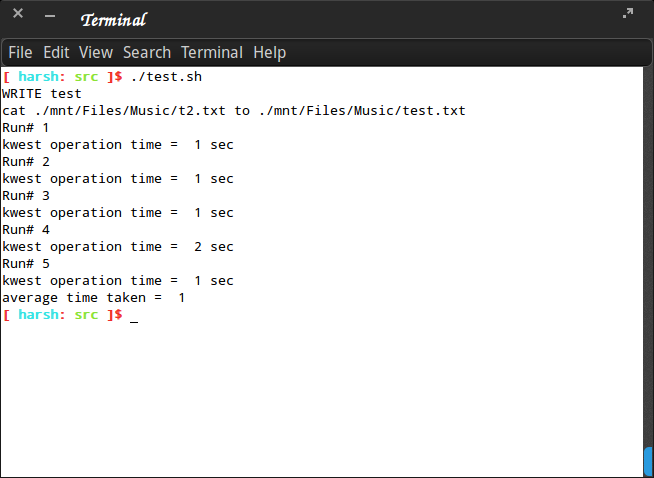
\includegraphics[width=0.8\linewidth]{./opimg/writetest.png}}
%\includegraphics[width=0.8\textwidth]{image.png}
\caption{Write operation average time on 4.1MB text file}
\label{fig:dfd0}
\end{figure}


\subsection{Profiling Code}
Code can be profiled using Manual methods, or using specific tools such as Valgrind, GDB, Splint etc. For testing KWEST, we have used the following profiling tools:
\subsection*{GDB}
GDB can be used to debug the file system and check for memory leaks, errors and irregular operations. The sample output given below shows a clean mount and unmount of the KWEST file system.
\begin{lstlisting}[language=bash,frame=single]
$ gdb ./kwest
GNU gdb (GDB) 7.5-ubuntu
Copyright (C) 2012 Free Software Foundation, Inc.
Reading symbols from kwest/src/kwest....
(gdb) run -s -d -f mnt
Starting program: kwest/src/kwest -s -d -f mnt
[Thread debugging using libthread_db enabled]
Using host libthread_db library "/lib/x86_64-linux-gnu/libthread_db.so.1".
KWEST - A Semantically Tagged Virtual File System
...
...
[Inferior 1 (process 20863) exited normally]
(gdb) bt
No stack.
\end{lstlisting}

Using GDB, we can test the file system and record the various errors occuring under testing. The following table depicts each file system operation and the possible errors occuring on it - \\

\begin{tabular}{|p{3cm}|p{2cm}|p{8cm}|}
\hline
\textbf{Test} & \textbf{Status} & \textbf{Possible Errors} \\ \hline
list directory	&	PASS &  I/O error, illegal operation, transport endpoint not connection, connection abort \\ \hline
read file & PASS & I/O error, illegal operation, access denied, database error \\ \hline
write file & PASS & I/O error, illegal operation, access denied, file system busy \\ \hline
mknod & PASS & Operation not permitted, I/O error, database error \\ \hline
unlink & PASS & Device busy, Operation not permitted, I/O error, database error \\ \hline
mkdir & PASS & Operation not permitted, I/O error, database error \\ \hline
rmdir & PASS & Device busy, Operation not permitted, I/O error, database error \\ \hline
chmod & PASS & Access denied, I/O error, device busy, database error \\ \hline
associations & PASS & memory error, segmentation fault, unconditional jump, I/O error \\ \hline
fuse main & PASS & incompatible version \\
\hline
\end{tabular}
\captionof{table}{GDB debugging for KWEST}

